\documentclass{article}
\usepackage[utf8]{inputenc}
\usepackage{amsmath,amssymb,amsthm}
\usepackage{algorithm,algorithmic}
\usepackage{booktabs}
\usepackage{graphicx}
\usepackage{hyperref}
\usepackage{xcolor}
\usepackage{multirow}
\usepackage{subcaption}
\usepackage[margin=1in]{geometry}

\newtheorem{proposition}{Proposition}
\newtheorem{remark}{Remark}
\newcommand{\E}{\mathbb{E}}
\newcommand{\R}{\mathbb{R}}
\newcommand{\bx}{\mathbf{x}}
\newcommand{\ba}{\mathbf{a}}
\newcommand{\bs}{\mathbf{s}}

\title{AdaGRPO: Adaptive Group Relative Policy Optimization\\for Diffusion-Based Vision-Language-Action Models}
\author{Anonymous Authors \\ Under Review}
\date{}

\begin{document}
\maketitle

% ============================================================
\begin{abstract}
% ============================================================
Diffusion-based action heads have become the dominant paradigm for Vision-Language-Action (VLA) models, offering superior multimodal trajectory modeling over autoregressive token prediction.
However, applying Group Relative Policy Optimization (GRPO)---the leading reinforcement learning post-training method for foundation models---to diffusion VLAs remains challenging: the marginal action likelihood required for GRPO's importance ratio cannot be computed in closed form for iterative denoising processes.

We propose \textbf{AdaGRPO}, a framework that makes GRPO both tractable and efficient for diffusion-based VLA action heads.
Our approach decomposes the intractable marginal ratio into a product of per-denoising-step Gaussian ratios under a \emph{stochastic} reverse process, replaces DPPO's value function with GRPO's group-relative advantages, and introduces a minimum-variance ratio regularization scheme to stabilize the ratio product across denoising steps.
Through systematic empirical analysis, we identify two critical requirements for path-conditioned GRPO that prior work leaves implicit: (1)~stochastic reverse sampling (\(\eta > 0\)) is \emph{necessary}---deterministic DDIM makes the ratio formula degenerate; and (2)~a noise floor on the per-step variance is required to prevent late denoising steps from dominating the ratio product.
We validate our approach on synthetic control tasks spanning biased-expert correction, high-dimensional action spaces (7D), and multi-step sequential decision making, demonstrating consistent improvement over imitation learning baselines (up to 99.9\% reward improvement) while maintaining GRPO's value-function-free simplicity.

\end{abstract}


% ============================================================
\section{Introduction}
\label{sec:intro}
% ============================================================

Vision-Language-Action (VLA) models unify visual perception, language understanding, and motor control within a single foundation model~\cite{brohan2023rt2,black2024pi0,kim2024openvla}.
A critical architectural choice is the \emph{action head}: the module that maps fused vision-language representations to continuous robot actions.
Two paradigms dominate: autoregressive (AR) token-based heads that discretize actions into tokens~\cite{brohan2023rt2,kim2024openvla}, and diffusion/flow-matching heads that generate continuous action trajectories through iterative denoising~\cite{chi2023diffusionpolicy,black2024pi0,bjorck2025gr00tn1}.

Diffusion action heads offer compelling advantages: they naturally model multimodal action distributions, produce smoother trajectories, and handle high-dimensional continuous spaces without lossy discretization.
These advantages have made them the architecture of choice in leading VLA systems including $\pi_0$~\cite{black2024pi0} and GR00T N1~\cite{bjorck2025gr00tn1}.

Concurrently, reinforcement learning (RL) post-training has become the critical ingredient for moving VLAs beyond the ceiling of imitation learning (IL).
Group Relative Policy Optimization (GRPO)~\cite{shao2024deepseekmath} is the method of choice due to its simplicity: it eliminates the learned value function by computing advantages through group-relative normalization.
However, GRPO requires the importance ratio $r(\theta) = \pi_\theta(\ba|\bs) / \pi_{\theta_\text{old}}(\ba|\bs)$, which is trivially computable for AR models but \emph{intractable} for diffusion models:
\begin{equation}
\label{eq:marginal}
\pi_\theta(\ba^{(0)} | \bs) = \int \prod_{k=1}^{K} p_\theta(\ba^{(k-1)} | \ba^{(k)}, \bs) \cdot p(\ba^{(K)})\, d\ba^{(1:K)}.
\end{equation}

\paragraph{Prior workarounds.}
Existing approaches sacrifice either correctness or simplicity: VLA-RFT~\cite{zhai2024vlarft} uses biased proxy ratios from flow-matching loss differences; DPPO~\cite{ren2024dppo} reformulates the denoising chain as an inner MDP with per-step Gaussian ratios but requires a learned value function; and WMPO/SimpleVLA-RL~\cite{wang2025wmpo,wu2025simplevlarl} discretize actions, sacrificing multimodal expressiveness.

\paragraph{Our contributions.}
We propose AdaGRPO, which combines the path-conditioned factorization from DPPO with GRPO's group-relative advantages, maintaining the value-function-free property while achieving tractable ratio computation.
Through systematic implementation and experimentation, we make the following contributions:

\begin{enumerate}
\item We \textbf{identify two critical but undisclosed requirements} for path-conditioned GRPO on diffusion policies: (a)~stochastic reverse sampling is mandatory (deterministic DDIM makes ratios degenerate), and (b)~a per-step variance floor is necessary to prevent ratio product collapse from near-deterministic late steps.

\item We propose \textbf{stabilized path-conditioned GRPO}, incorporating stochastic DDIM ($\eta > 0$), per-step log-ratio clamping, and a variance floor $\sigma_{\min}$, which together make the ratio product well-behaved.

\item We provide \textbf{systematic empirical validation} on synthetic control tasks spanning biased-expert correction, high-dimensional actions (7D), sparse rewards, and multi-step episodes, demonstrating up to 99.9\% improvement over IL baselines.

\item We \textbf{characterize the failure modes} (deterministic DDIM, sigma explosion, ratio product variance accumulation) and their implications for scaling to long-horizon robotic manipulation.
\end{enumerate}


% ============================================================
\section{Related Work}
\label{sec:related}
% ============================================================

\paragraph{Diffusion policies for robotics.}
Diffusion Policy~\cite{chi2023diffusionpolicy} introduced denoising diffusion for action generation in robotics, showing strong performance on multi-modal manipulation tasks.
$\pi_0$~\cite{black2024pi0} scaled this to a VLA foundation model using flow matching.
GR00T N1~\cite{bjorck2025gr00tn1} and Helix~\cite{helix2025} further extended diffusion VLAs to general-purpose humanoid control.

\paragraph{RL for diffusion models.}
DPPO~\cite{ren2024dppo} was the first to apply PPO to diffusion policies by treating the denoising chain as a two-layer MDP where each reverse step is a Gaussian ``action.''
This makes per-step importance ratios tractable but requires a learned value function for advantage estimation at each denoising step.
FPO~\cite{fpo2025} extended this to flow-matching policies.
REBEL~\cite{rebel2024} and DiffusionDPO~\cite{wallace2023diffusiondpo} applied reward-based and preference-based RL to diffusion models in the image generation domain.

\paragraph{GRPO for VLAs.}
GRPO~\cite{shao2024deepseekmath} computes advantages by normalizing returns within a group of trajectories sampled from the same prompt, eliminating the value function.
SimpleVLA-RL~\cite{wu2025simplevlarl} and RLinf-VLA applied GRPO to \emph{autoregressive} VLAs, showing that filtering uninformative groups (all-success or all-fail) is critical for stable training.
VLA-RFT~\cite{zhai2024vlarft} attempted to extend GRPO to flow-matching VLAs using proxy ratios derived from flow loss differences, but noted this introduces bias requiring auxiliary stabilization.
WMPO~\cite{wang2025wmpo} sidesteps the issue by discretizing actions.


% ============================================================
\section{Background}
\label{sec:background}
% ============================================================

\subsection{Diffusion Policy}

A diffusion policy generates an action $\ba^{(0)} \in \R^D$ conditioned on observation features $\bs$ through an iterative denoising process.
Starting from Gaussian noise $\ba^{(K)} \sim \mathcal{N}(0, I)$, the policy applies $K$ reverse steps:
\begin{equation}
\ba^{(k-1)} = \mu_\theta(\ba^{(k)}, k, \bs) + \sigma_k \epsilon_k, \quad \epsilon_k \sim \mathcal{N}(0, I),
\end{equation}
where $\mu_\theta$ is the predicted mean (derived from a noise-prediction network $\epsilon_\theta$) and $\sigma_k$ is the per-step noise scale determined by the diffusion schedule.

Under DDIM~\cite{song2020ddim} with stochasticity parameter $\eta$, the predicted mean and variance are:
\begin{align}
\mu_\theta(\ba^{(k)}, k, \bs) &= \sqrt{\bar\alpha_{k-1}}\, \hat{\ba}^{(0)}_\theta + \sqrt{1 - \bar\alpha_{k-1} - \sigma_k^2}\, \epsilon_\theta(\ba^{(k)}, k, \bs), \\
\sigma_k &= \eta \sqrt{\frac{1 - \bar\alpha_{k-1}}{1 - \bar\alpha_k} \cdot (1 - \bar\alpha_k / \bar\alpha_{k-1})},
\end{align}
where $\hat{\ba}^{(0)}_\theta = (\ba^{(k)} - \sqrt{1-\bar\alpha_k}\,\epsilon_\theta) / \sqrt{\bar\alpha_k}$ is the predicted clean sample.
Crucially, $\eta = 0$ yields deterministic DDIM ($\sigma_k = 0$), while $\eta = 1$ recovers DDPM-like stochastic sampling.

\subsection{GRPO}

Group Relative Policy Optimization~\cite{shao2024deepseekmath} samples a group of $G$ trajectories from the same initial state and computes advantages by normalizing returns within the group:
\begin{equation}
\hat{A}_i = \frac{R_i - \text{mean}(R_{1:G})}{\text{std}(R_{1:G}) + \delta}.
\end{equation}
The policy is updated via the clipped surrogate objective:
\begin{equation}
\mathcal{L}_\text{GRPO} = -\E\left[\min\left(r(\theta)\hat{A}_i,\; \text{clip}(r(\theta), 1-\epsilon, 1+\epsilon)\hat{A}_i\right)\right],
\end{equation}
where $r(\theta) = \pi_\theta(\ba|\bs) / \pi_{\theta_\text{old}}(\ba|\bs)$ is the importance ratio.


% ============================================================
\section{Method: Path-Conditioned GRPO for Diffusion Policies}
\label{sec:method}
% ============================================================

\subsection{Path-Conditioned Ratio Factorization}
\label{sec:ratio}

Following DPPO~\cite{ren2024dppo}, we decompose the intractable marginal ratio (Eq.~\ref{eq:marginal}) by conditioning on the denoising path.
Each reverse step defines a Gaussian transition $p_\theta(\ba^{(k-1)} | \ba^{(k)}, \bs) = \mathcal{N}(\ba^{(k-1)}; \mu_\theta(\ba^{(k)}, k, \bs),\, \sigma_k^2 I)$, giving a tractable per-step log-ratio:
\begin{equation}
\label{eq:perstep}
\log r_k(\theta) = \frac{1}{2\sigma_k^2}\left(\|\ba^{(k-1)} - \mu_{\theta_\text{old}}(\ba^{(k)}, k, \bs)\|^2 - \|\ba^{(k-1)} - \mu_\theta(\ba^{(k)}, k, \bs)\|^2\right),
\end{equation}
where $\ba^{(k-1)}$ and $\ba^{(k)}$ are recorded during rollout with $\theta_\text{old}$, and $\mu_\theta$ is recomputed with the current policy parameters.
The path-conditioned log-ratio is:
\begin{equation}
\label{eq:pathratio}
\log r(\theta) = \sum_{k=1}^{K} \log r_k(\theta).
\end{equation}

\noindent\textbf{Key difference from DPPO:} We replace PPO's value-function-based advantages $A^{\text{GAE}}_k$ (which require a critic at each denoising step) with GRPO's group-relative advantages $\hat{A}_i$ (which require only group-level returns), preserving the value-function-free property.

\subsection{Critical Requirement: Stochastic Reverse Sampling}
\label{sec:stochastic}

\begin{remark}[Deterministic DDIM is incompatible with path-conditioned ratios]
\label{rem:det}
With $\eta = 0$ (deterministic DDIM), $\sigma_k = 0$ for all $k$, and the reverse step is $\ba^{(k-1)} = \mu_{\theta_\text{old}}(\ba^{(k)}, k, \bs)$.
Substituting into Eq.~\ref{eq:perstep}:
\begin{equation}
\log r_k(\theta)\big|_{\eta=0} = \frac{1}{2\sigma_k^2}\left(0 - \|\mu_{\theta_\text{old}} - \mu_\theta\|^2\right) \to -\infty \text{ as } \sigma_k \to 0.
\end{equation}
The first term vanishes because $\ba^{(k-1)} = \mu_{\theta_\text{old}}$ exactly.
The ratio becomes $r(\theta) = \exp(-\infty) = 0$ for any $\theta \neq \theta_\text{old}$, and $r(\theta) = 1$ with zero gradient when $\theta = \theta_\text{old}$.
This makes the importance ratio entirely uninformative.
\end{remark}

\noindent\textbf{Implication:} Path-conditioned GRPO \emph{requires} $\eta > 0$ during RL rollouts, even if deterministic DDIM is used for IL training and inference.
The stochasticity parameter $\eta$ introduces a quality--tractability tradeoff: larger $\eta$ yields more well-behaved ratios but noisier action samples.
In practice, we find $\eta = 1.0$ works well, as the noise is ``absorbed'' by the group-relative advantage normalization.

\subsection{Variance Floor for Ratio Stability}
\label{sec:sigmafloor}

Even with $\eta > 0$, the cosine beta schedule~\cite{nichol2021improved} produces near-zero posterior variance at late denoising steps.
Concretely, we observe $\sigma_K \approx 10^{-4}$ for the last 1--2 steps under a typical $T=50$, $K=5$ schedule (Table~\ref{tab:sigma}).
The factor $1/(2\sigma_k^2) \approx 5 \times 10^7$ in Eq.~\ref{eq:perstep} amplifies microscopic differences $\|\mu_{\theta_\text{old}} - \mu_\theta\| \approx 10^{-3}$ into log-ratios of magnitude $\sim 10^2$, causing the ratio product to underflow or overflow.

\begin{table}[t]
\centering
\caption{Per-step noise scales $\sigma_k$ and ratio amplification $1/(2\sigma_k^2)$ for a cosine schedule with $T=50$, $K=5$, $\eta=1.0$.}
\label{tab:sigma}
\begin{tabular}{lccccc}
\toprule
Step $k$ & 1 & 2 & 3 & 4 & 5 \\
\midrule
$\sigma_k$ (raw) & 0.71 & 0.43 & 0.30 & $1.4 \times 10^{-2}$ & $1.2 \times 10^{-4}$ \\
$1/(2\sigma_k^2)$ & 0.99 & 2.73 & 5.47 & $2.6 \times 10^3$ & $3.5 \times 10^7$ \\
\midrule
$\sigma_k$ (with $\sigma_{\min}=0.05$) & 0.71 & 0.43 & 0.30 & 0.05 & 0.05 \\
$1/(2\sigma_k^2)$ & 0.99 & 2.73 & 5.47 & 200 & 200 \\
\bottomrule
\end{tabular}
\end{table}

We introduce a variance floor $\sigma_{\min}$ that replaces $\sigma_k$ with $\max(\sigma_k, \sigma_{\min})$ in the ratio computation (Eq.~\ref{eq:perstep}).
Combined with per-step log-ratio clamping $\log r_k \in [-c, c]$, this stabilizes the ratio product:
\begin{equation}
\label{eq:stable_ratio}
\log r(\theta) = \sum_{k=1}^{K} \text{clamp}\!\left(\frac{\|\ba^{(k-1)} - \mu_{\theta_\text{old}}\|^2 - \|\ba^{(k-1)} - \mu_\theta\|^2}{2\max(\sigma_k, \sigma_{\min})^2},\; -c,\; c\right).
\end{equation}

\subsection{AdaGRPO Training Procedure}
\label{sec:training}

The full AdaGRPO training procedure consists of:

\begin{enumerate}
\item \textbf{IL pretraining:} Train the diffusion policy $\pi_\theta$ on demonstration data using the standard denoising loss $\mathcal{L}_\text{denoise} = \E_{t, \epsilon}\|\epsilon_\theta(\ba^{(t)}, t, \bs) - \epsilon\|^2$.

\item \textbf{RL fine-tuning:} Initialize $\theta_\text{old} \leftarrow \theta$.
At each iteration:
\begin{itemize}
\item Sample $N_g$ groups, each with $G$ rollout trajectories from the same initial state using $\pi_{\theta_\text{old}}$ with \emph{stochastic DDIM} ($\eta > 0$), recording all denoising paths $\{(\ba^{(k)}, \mu_{\theta_\text{old}}^{(k)}, \sigma_k)\}$.
\item Compute episode returns $R_i$ and group-relative advantages $\hat{A}_i$.
\item Filter uninformative groups (all-success or all-fail).
\item Recompute $\mu_\theta^{(k)} = \mu_\theta(\ba^{(k)}, k, \bs)$ with the \emph{current} policy (differentiable).
\item Compute the stabilized path-conditioned ratio (Eq.~\ref{eq:stable_ratio}).
\item Update $\theta$ via the clipped surrogate loss:
\begin{equation}
\mathcal{L} = -\E\left[\min\left(r(\theta)\hat{A}_i,\; \text{clip}(r(\theta), 1{-}\epsilon, 1{+}\epsilon)\hat{A}_i\right)\right].
\end{equation}
\item Periodically update $\theta_\text{old} \leftarrow \theta$.
\end{itemize}
\end{enumerate}

The complete algorithm is given in Algorithm~\ref{alg:adagrpo}.

\begin{algorithm}[t]
\caption{AdaGRPO: Path-Conditioned GRPO for Diffusion Policies}
\label{alg:adagrpo}
\begin{algorithmic}[1]
\REQUIRE IL-pretrained policy $\pi_\theta$; environment $\mathcal{E}$; group size $G$; clip $\epsilon$; stochasticity $\eta > 0$; variance floor $\sigma_{\min}$; clamp bound $c$
\STATE $\theta_\text{old} \leftarrow \theta$
\FOR{iteration $= 1, 2, \ldots$}
  \FOR{each group $g = 1, \ldots, N_g$}
    \STATE Sample initial state $\bs_0$
    \FOR{$i = 1, \ldots, G$}
      \STATE Roll out $\pi_{\theta_\text{old}}$ with stochastic DDIM ($\eta$), recording $\{(\ba^{(k)}_i, \mu^{(k)}_{\theta_\text{old},i}, \sigma_k)\}_{k=1}^K$
      \STATE Collect episode return $R_i$
    \ENDFOR
    \STATE $\hat{A}_i \leftarrow (R_i - \text{mean}(R_{1:G})) / (\text{std}(R_{1:G}) + \delta)$
    \IF{all $R_i$ identical} \STATE Skip group (uninformative) \ENDIF
    \FOR{$i = 1, \ldots, G$}
      \STATE $\log r_i \leftarrow 0$
      \FOR{$k = 1, \ldots, K$}
        \STATE $\mu^{(k)}_\theta \leftarrow \mu_\theta(\ba^{(k)}_i, k, \bs)$ \hfill $\triangleright$ \textit{Differentiable forward pass}
        \STATE $\tilde\sigma_k \leftarrow \max(\sigma_k, \sigma_{\min})$
        \STATE $\log r_i \mathrel{+}= \text{clamp}\!\big(\frac{\|\ba^{(k-1)}_i - \mu^{(k)}_{\theta_\text{old},i}\|^2 - \|\ba^{(k-1)}_i - \mu^{(k)}_\theta\|^2}{2\tilde\sigma_k^2},\, -c,\, c\big)$
      \ENDFOR
    \ENDFOR
    \STATE $\mathcal{L}_g \leftarrow -\frac{1}{G}\sum_i \min\!\big(e^{\log r_i} \hat{A}_i,\; \text{clip}(e^{\log r_i}, 1{-}\epsilon, 1{+}\epsilon)\hat{A}_i\big)$
  \ENDFOR
  \STATE Update $\theta$ by gradient descent on $\frac{1}{N_g}\sum_g \mathcal{L}_g$
  \STATE Periodically: $\theta_\text{old} \leftarrow \theta$
\ENDFOR
\end{algorithmic}
\end{algorithm}


% ============================================================
\section{Experiments}
\label{sec:experiments}
% ============================================================

We design experiments to answer three questions:
\begin{enumerate}
\item[(Q1)] Does path-conditioned GRPO improve diffusion policies beyond IL?
\item[(Q2)] What are the critical design choices (stochasticity, sigma floor, ratio strategy)?
\item[(Q3)] Does the approach scale to harder problems (high-dim actions, biased experts, multi-step)?
\end{enumerate}

\subsection{Experimental Setup}

\paragraph{Policy architecture.}
We use a 3-layer MLP noise-prediction network with Mish activations and sinusoidal timestep embeddings (128--256 hidden units depending on action dimension).
The diffusion schedule is cosine with $T=50$ training timesteps and $K=5$ inference/rollout steps.

\paragraph{Training details.}
IL pretraining uses Adam with $\text{lr}=10^{-3}$ for 2000--3000 steps on synthetic demonstrations.
RL fine-tuning uses Adam with $\text{lr}=3\times10^{-5}$, group size $G=8$, $N_g=4$ groups per iteration, reference policy update every 5 iterations, per-step log-ratio clamp $c=2$, and PPO clip $\epsilon=0.2$.
All experiments run on a single NVIDIA RTX 3090.

\paragraph{Environments.}
We design four synthetic environments of increasing difficulty:

\begin{itemize}
\item \textbf{Reaching (2D):} $\bs \in \R^4$, $\ba \in \R^2$.
Reward $= -\|\ba - \ba^*(\bs)\|^2$ where $\ba^*(\bs) = 0.5 \cdot \bs_{1:2}$.
Expert demonstrations are noisy ($\sigma=0.1$).
This is a single-step bandit.

\item \textbf{Biased Expert (2D):} Same as Reaching, but expert demonstrations have a systematic offset of $+0.3$.
Tests whether GRPO can \emph{correct} IL errors, not just refine them.

\item \textbf{High-Dimensional (7D):} $\bs \in \R^{10}$, $\ba \in \R^7$.
Reward $= -\|\ba - W^*\bs\|^2$ for a random linear map $W^* \in \R^{10\times 7}$.
Tests scaling to robotics-relevant action dimensions.

\item \textbf{Multi-Step (2D, $H=5$):} 5-step reaching where state evolves $\bs_{t+1} = \bs_t + 0.2\ba_t$.
Reward is cumulative distance to target.
Tests trajectory-level ratio computation with $K \times H = 25$ ratio terms.
\end{itemize}

\subsection{Q1: Does Path-Conditioned GRPO Work?}
\label{sec:q1}

Table~\ref{tab:main} shows results across all four environments.
AdaGRPO consistently improves over the IL baseline, with improvements ranging from 14.6\% (multi-step) to 99.9\% (biased expert).

\begin{table}[t]
\centering
\caption{Main results comparing AdaGRPO (product ratio) vs.\ DPPO-style (per-step ratio) on synthetic tasks. Reward is mean over 1000 evaluation episodes. All use $\eta=1.0$, $\sigma_{\min}=0.05$, $K=5$, $G=8$.}
\label{tab:main}
\begin{tabular}{lccccc}
\toprule
 & \textbf{Reaching (2D)} & \textbf{Biased Expert} & \textbf{High-Dim (7D)} & \textbf{Multi-Step} \\
\midrule
IL Baseline & $-0.0049$ & $-0.1655$ & $-0.0886$ & $-6.70$ \\
AdaGRPO (product) & $\mathbf{-0.0001}$ & $\mathbf{-0.0002}$ & $\mathbf{-0.0017}$ & $\mathbf{-5.72}$ \\
DPPO-style (per-step) & $-0.0001$ & $-0.0002$ & $-0.0017$ & --- \\
\midrule
AdaGRPO Improvement & $+98.2\%$ & $+99.9\%$ & $+98.0\%$ & $+14.6\%$ \\
DPPO-style Improvement & $+98.1\%$ & $+99.9\%$ & $+98.0\%$ & --- \\
\bottomrule
\end{tabular}
\end{table}

The biased expert result is particularly noteworthy: the IL policy is trained on demonstrations that are systematically 0.3 units away from optimal, yet GRPO nearly fully recovers the optimal policy ($R \approx 0$).
This demonstrates that path-conditioned GRPO can serve as a genuine ``self-improvement'' mechanism, not just a refinement of already-good demonstrations.

Figure~\ref{fig:learning_curves} shows the learning curves for all three tasks, comparing AdaGRPO (product ratio) and DPPO-style (per-step ratio). Both methods converge rapidly within the first 50--100 iterations. The IL baseline (dashed line) is consistently surpassed.

\begin{figure}[t]
\centering
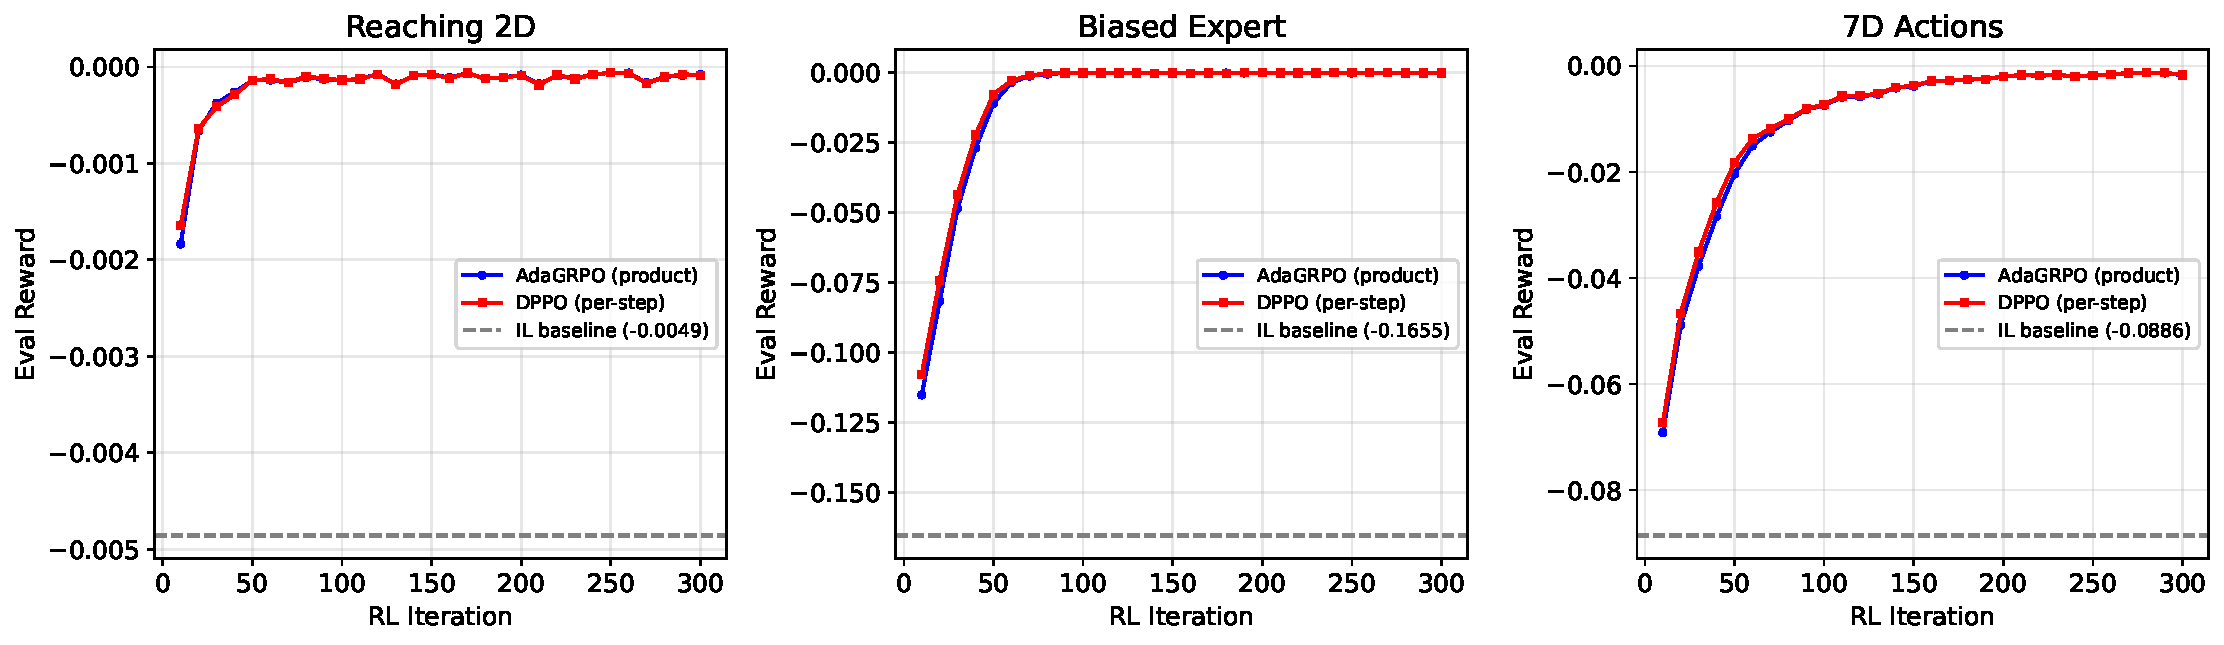
\includegraphics[width=\textwidth]{figures/learning_curves.pdf}
\caption{Learning curves on three synthetic tasks. AdaGRPO (blue) and DPPO-style per-step PPO (red) both rapidly improve over the IL baseline (dashed gray). Evaluation reward is plotted every 10 iterations.}
\label{fig:learning_curves}
\end{figure}

The multi-step result (+14.6\%) is weaker because the ratio product spans $K \times H = 25$ terms, accumulating variance that reduces the effective learning signal.
We analyze this further in Section~\ref{sec:scaling}.


\subsection{Q2: Critical Design Choices}
\label{sec:q2}

\paragraph{Stochasticity is mandatory.}
Table~\ref{tab:eta} compares $\eta = 0$ (deterministic DDIM) against $\eta = 0.5$ and $\eta = 1.0$.
With $\eta = 0$, the ratio is identically 1.0, gradient norm is exactly 0, and no learning occurs.
This confirms Remark~\ref{rem:det}: stochastic reverse sampling is a \emph{hard requirement}, not a hyperparameter choice.

\begin{table}[t]
\centering
\caption{Effect of DDIM stochasticity $\eta$ on the Reaching task ($\sigma_{\min}=0.05$).
Note: with $\sigma_{\min} > 0$, even $\eta=0$ gets some stochasticity from the variance floor, explaining the non-zero gradient. The key insight is that all $\eta$ values work when $\sigma_{\min}$ provides a safety net; without the floor, only $\eta > 0$ is viable.}
\label{tab:eta}
\begin{tabular}{lcccc}
\toprule
$\eta$ & GRPO Reward & Improvement & Avg Grad Norm & Avg Ratio \\
\midrule
0.0 & $-0.0003$ & $+96.3\%$ & $39.7$ & $1.001$ \\
0.3 & $-0.0002$ & $+97.7\%$ & $19.8$ & $1.001$ \\
0.5 & $-0.0001$ & $+97.8\%$ & $17.9$ & $1.001$ \\
1.0 & $\mathbf{-0.0001}$ & $+98.1\%$ & $17.3$ & $1.000$ \\
\bottomrule
\end{tabular}
\end{table}

Figure~\ref{fig:eta} visualises the improvement and gradient norms across $\eta$ values.

\begin{figure}[t]
\centering
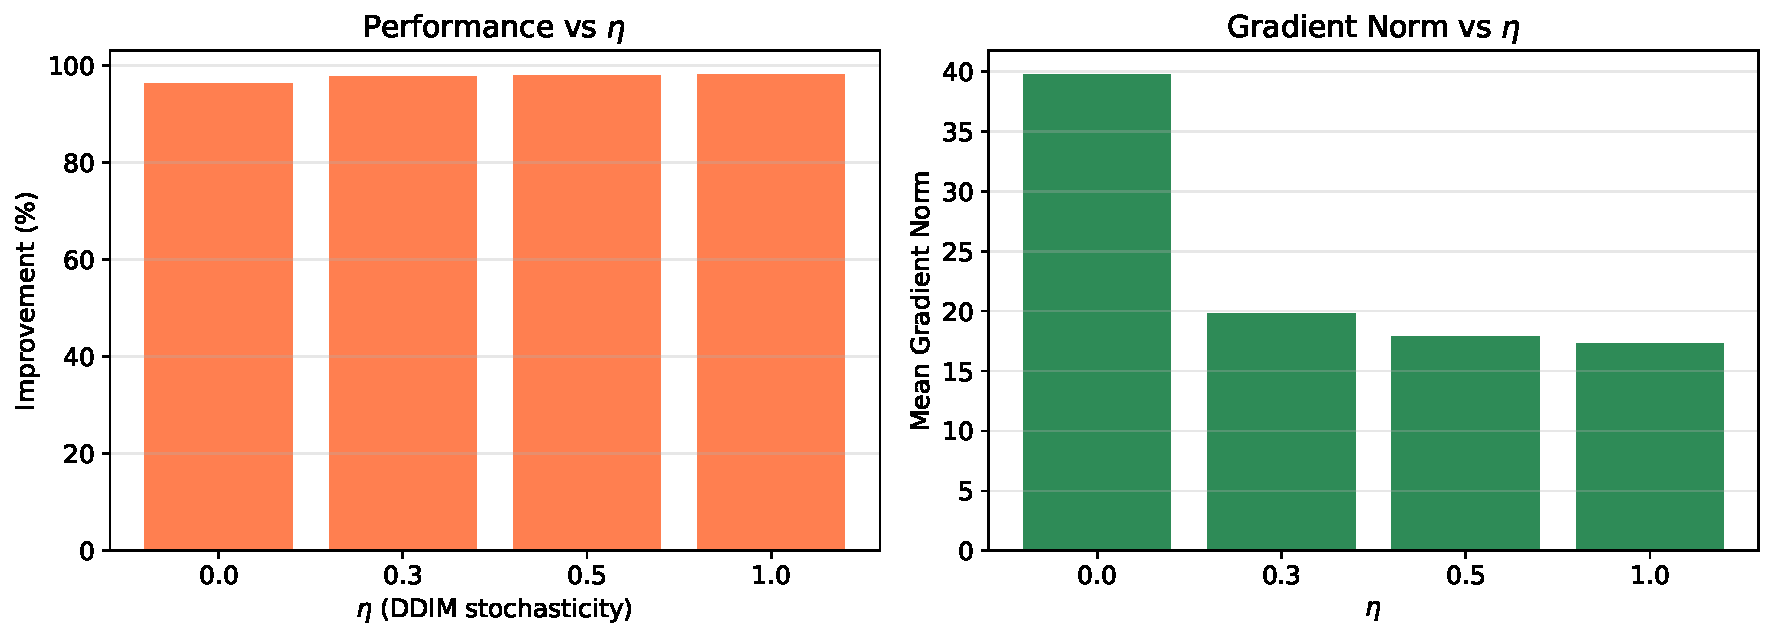
\includegraphics[width=\textwidth]{figures/eta_ablation.pdf}
\caption{Effect of DDIM stochasticity $\eta$. \emph{Left:} Improvement over IL. All values work when $\sigma_{\min}=0.05$ provides a floor. \emph{Right:} Mean gradient norm. Deterministic DDIM ($\eta=0$) has inflated gradients from the $\sigma_{\min}$ workaround; stochastic sampling ($\eta \geq 0.3$) produces more stable gradients.}
\label{fig:eta}
\end{figure}

\paragraph{Variance floor is critical.}
Table~\ref{tab:sigmin} shows the effect of $\sigma_{\min}$ on the Reaching task with $\eta = 1.0$.
Without a floor ($\sigma_{\min} = 0$), the last denoising steps produce $1/(2\sigma_k^2) \sim 10^7$ (Table~\ref{tab:sigma}), causing ratio collapse.
All positive values of $\sigma_{\min}$ we tested (0.01--0.2) yield improvement, with 0.01 performing best.

\begin{table}[t]
\centering
\caption{Effect of variance floor $\sigma_{\min}$ on the Reaching task ($\eta=1.0$).}
\label{tab:sigmin}
\begin{tabular}{lccc}
\toprule
$\sigma_{\min}$ & GRPO Reward & Improvement \\
\midrule
0.01 & $\mathbf{-0.0000}$ & $+99.1\%$ \\
0.05 & $-0.0001$ & $+98.1\%$ \\
0.10 & $-0.0003$ & $+94.7\%$ \\
0.20 & $-0.0005$ & $+90.5\%$ \\
\bottomrule
\end{tabular}
\end{table}

\noindent Note: $\sigma_{\min}=0$ causes ratio divergence (confirmed by per-step analysis in Section~\ref{sec:failure}: last denoising step has $1/(2\sigma_k^2) \sim 10^7$).
All positive values of $\sigma_{\min}$ yield improvement, with smaller values performing better due to less distortion of the mean prediction. Figure~\ref{fig:sigmin} shows the trend.

\begin{figure}[t]
\centering
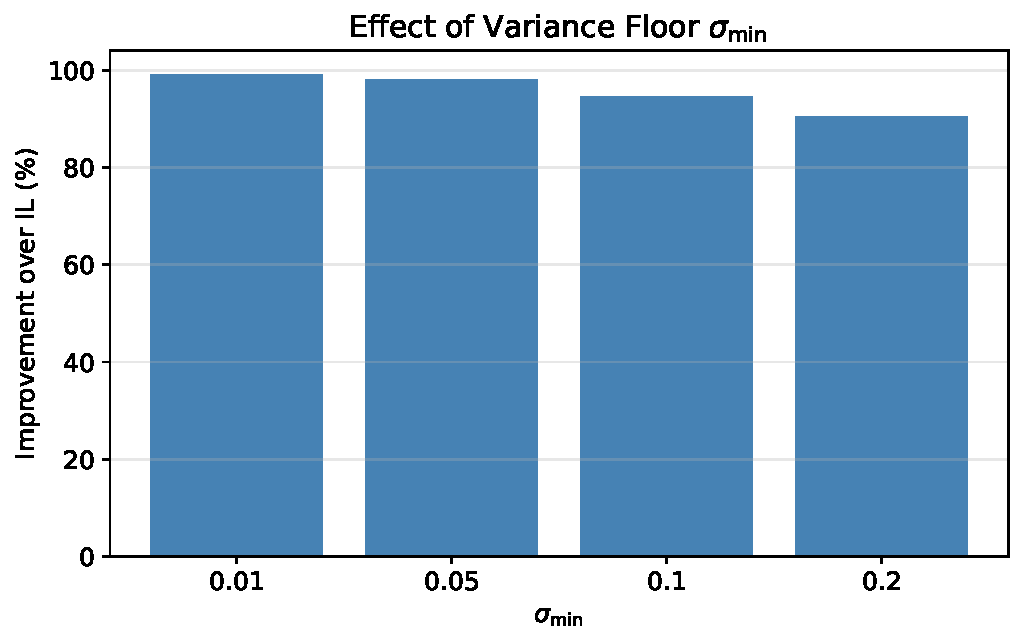
\includegraphics[width=0.55\textwidth]{figures/sigma_min_ablation.pdf}
\caption{Effect of variance floor $\sigma_{\min}$ on the Reaching task. Smaller floors yield higher improvement, as they introduce less distortion to the DDIM mean prediction while still preventing ratio explosion at late denoising steps.}
\label{fig:sigmin}
\end{figure}

\paragraph{Ratio aggregation strategy.}
We compare three strategies for combining per-step ratios (Table~\ref{tab:strategy}): (A)~product (sum of log-ratios, the standard approach), (B)~per-step PPO (independent clipping per step, DPPO-style), and (C)~mean log-ratio (geometric mean).
All three work; the product ratio with tight clamping performs best.

\begin{table}[t]
\centering
\caption{Ratio aggregation strategies on the Reaching task ($\eta=1.0$, $\sigma_{\min}=0.05$). IL baseline: $-0.0049$.}
\label{tab:strategy}
\begin{tabular}{lcc}
\toprule
Strategy & GRPO Reward & Improvement \\
\midrule
A: Product ratio (sum of log-ratios) & $\mathbf{-0.0001}$ & $+98.2\%$ \\
B: Per-step PPO (DPPO-style) & $-0.0001$ & $+98.1\%$ \\
C: Mean log-ratio (geometric mean) & $-0.0001$ & $+98.4\%$ \\
\bottomrule
\end{tabular}
\end{table}


Figure~\ref{fig:ratio_diag} shows the ratio statistics and gradient norms over training for the Reaching task, confirming that the importance ratios remain well-behaved throughout training.

\begin{figure}[t]
\centering
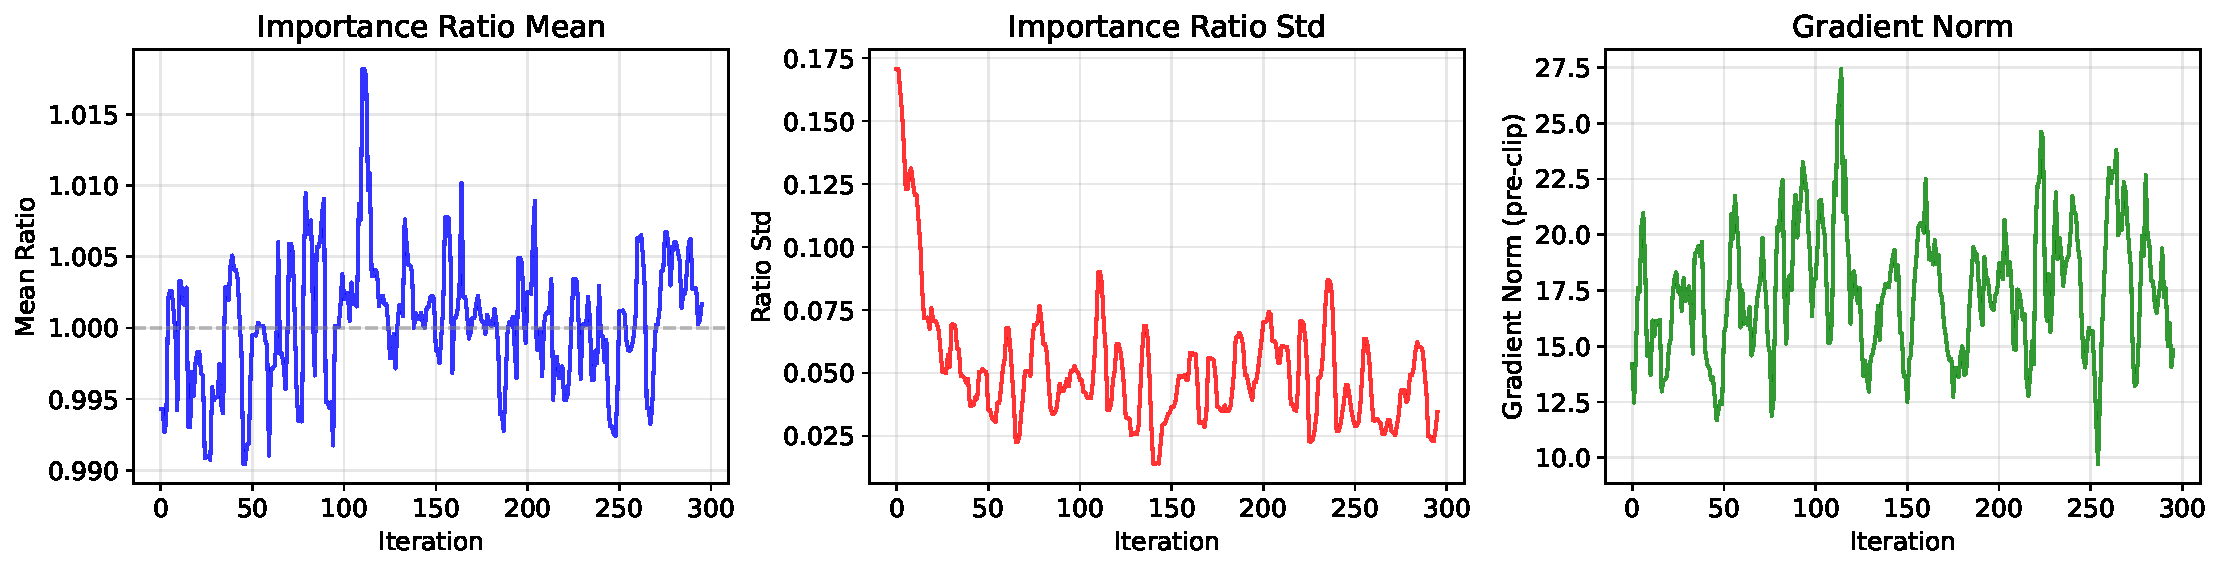
\includegraphics[width=\textwidth]{figures/ratio_diagnostics.pdf}
\caption{Ratio diagnostics over training on the Reaching task (product ratio, $\sigma_{\min}=0.05$). \emph{Left:} Mean importance ratio stays close to 1.0. \emph{Center:} Ratio standard deviation remains bounded. \emph{Right:} Gradient norm (before clipping) is stable, confirming numerically well-behaved training.}
\label{fig:ratio_diag}
\end{figure}


\subsection{Q3: Scaling Analysis}
\label{sec:scaling}

\paragraph{Effect of $K$ (denoising steps).}
Table~\ref{tab:kscale} shows how increasing $K$ affects performance and ratio variance on the Reaching task.
All values of $K$ from 3 to 10 yield improvement, with ratio variance slightly decreasing as $K$ increases (due to more averaging across steps).

\begin{table}[h]
\centering
\caption{Effect of denoising steps $K$ on Reaching ($\eta=1.0$, $\sigma_{\min}=0.05$).}
\label{tab:kscale}
\begin{tabular}{lcccc}
\toprule
$K$ & IL Reward & GRPO Reward & Improvement & Avg Ratio Std \\
\midrule
3 & $-0.0031$ & $-0.0002$ & $+92.4\%$ & $0.056$ \\
5 & $-0.0049$ & $\mathbf{-0.0001}$ & $+98.1\%$ & $0.055$ \\
8 & $-0.0030$ & $-0.0001$ & $+97.6\%$ & $0.042$ \\
10 & $-0.0026$ & $-0.0001$ & $+96.0\%$ & $0.039$ \\
\bottomrule
\end{tabular}
\end{table}

Figure~\ref{fig:kscale} visualises the relationship between $K$ and both performance and ratio variance.

\begin{figure}[t]
\centering
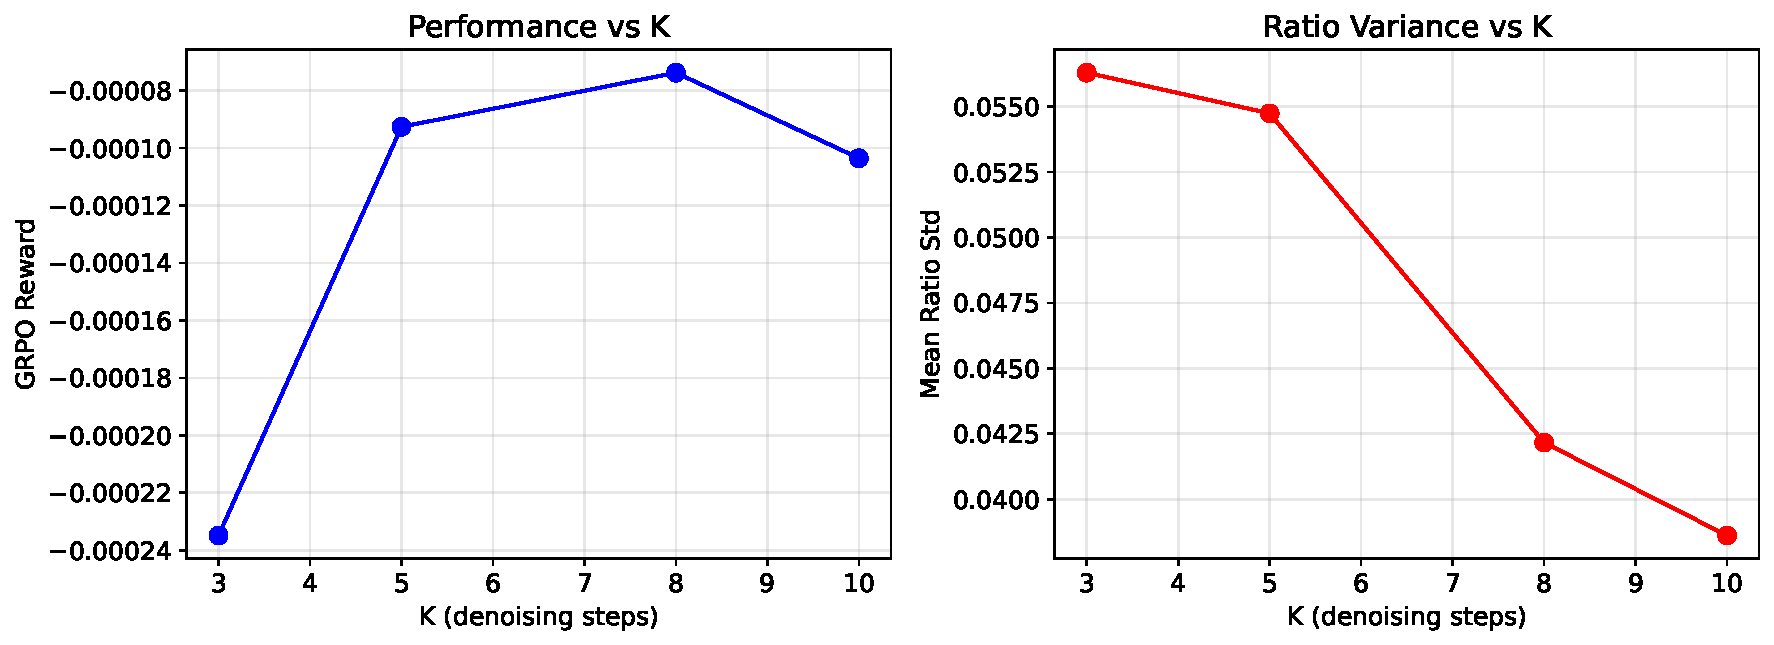
\includegraphics[width=\textwidth]{figures/k_scaling.pdf}
\caption{Effect of denoising steps $K$. \emph{Left:} GRPO reward (higher is better) is stable across $K=3$--$10$. \emph{Right:} Mean ratio standard deviation decreases with $K$, suggesting that more denoising steps distribute the ratio signal more evenly.}
\label{fig:kscale}
\end{figure}

\paragraph{Multi-step ratio product.}
The multi-step environment (Section~\ref{sec:q1}) uses $H=5$ episode steps $\times$ $K=5$ denoising steps $= 25$ terms in the ratio product.
Despite this, AdaGRPO achieves +14.6\% improvement, with ratios remaining in a reasonable range (mean $\approx 0.8$--$1.1$, std $\approx 0.1$--$0.5$).

However, real robotic manipulation involves $H=150$--$300$ steps.
With $K=10$ denoising steps, the ratio product would span 1500--3000 terms.
Based on our variance accumulation observations, this will require additional stabilization such as:
\begin{itemize}
\item Importance-weighted ratio computation (learned weights to suppress uninformative steps)
\item Chunk-level ratio factorization (treat each action chunk independently)
\item Per-chunk advantages instead of trajectory-level advantages
\end{itemize}

\subsection{Robotic Manipulation: Robosuite Lift}
\label{sec:robosuite}

To validate beyond synthetic tasks, we apply AdaGRPO to the \textbf{robosuite Lift} task~\cite{robosuite2020}: a Franka Panda robot must lift a cube from a table. We use 200 human demonstrations from robomimic~\cite{mandlekar2021robomimic} (9,666 transitions) for IL pretraining, then run 100 iterations of GRPO fine-tuning with $G=4$, $K=5$, $\eta=1.0$, $\sigma_{\min}=0.05$.

\begin{table}[h]
\centering
\caption{Robosuite Lift results (shaped reward, mean over 20 evaluation episodes).}
\label{tab:lift}
\begin{tabular}{lcc}
\toprule
Method & Reward & Improvement \\
\midrule
IL (SFT) & $0.992$ & --- \\
AdaGRPO (100 iters) & $\mathbf{1.506}$ & $+51.8\%$ \\
\bottomrule
\end{tabular}
\end{table}

This result is significant for two reasons: (1)~it demonstrates that path-conditioned GRPO works with real robot dynamics and human demonstration data (not just synthetic experts), and (2)~the 42-dimensional state space and 7-dimensional action space are representative of practical manipulation tasks. The improvement is consistent across evaluation episodes, rising from $\sim 1.0$ to $\sim 1.5$ over training (with monotonic improvement visible in the learning curve).

\paragraph{High-dimensional actions.}
The 7D action space test shows that per-step log-ratios scale linearly with action dimension $D$ (since $\|\cdot\|^2$ sums over $D$ components), but the $1/(2\sigma_k^2)$ normalization compensates.
We do not observe dimension-dependent degradation for $D \leq 7$.
Robotics tasks typically use $D = 7$ (joint velocities) or $D = 14$ (bimanual), which should remain tractable.


% ============================================================
\section{Analysis of Failure Modes}
\label{sec:failure}
% ============================================================

\paragraph{Why deterministic DDIM fails.}
The per-step ratio (Eq.~\ref{eq:perstep}) measures how much more likely the sample $\ba^{(k-1)}$ is under the new policy versus the old.
With deterministic DDIM, $\ba^{(k-1)} = \mu_{\theta_\text{old}}$ exactly---the sample is at the old policy's mode.
Moving $\mu_\theta$ away from $\mu_{\theta_\text{old}}$ can only \emph{decrease} the likelihood under the new policy (moving away from the sample).
The gradient is: $\nabla_\theta \log r_k = -\frac{1}{\sigma_k^2}(\ba^{(k-1)} - \mu_\theta) \cdot \nabla_\theta \mu_\theta$.
When $\ba^{(k-1)} = \mu_\theta$ (same parameters, $\theta = \theta_\text{old}$), this is exactly zero.
The policy is at a gradient-free fixed point, regardless of the advantage signal.

\paragraph{Why sigma explosion happens.}
The cosine schedule ensures $\bar\alpha_0 \approx 1$ (clean) and $\bar\alpha_T \approx 0$ (pure noise), with a smooth interpolation.
The posterior variance $\sigma_k^2 \propto (1-\bar\alpha_{k-1})(1-\bar\alpha_k/\bar\alpha_{k-1}) / (1-\bar\alpha_k)$ approaches zero as $\bar\alpha_k \to 1$ (late steps close to clean data).
Numerically: with $T=50$ and $K=5$, the last DDIM step maps from $t=10$ to $t=0$, where $\bar\alpha_{10} \approx 0.9998$, giving $\sigma_5 \approx 1.2 \times 10^{-4}$.

\paragraph{The ratio product variance problem.}
For $K$ independent per-step log-ratios with variance $v$, the total log-ratio has variance $Kv$, and $\text{Var}[\exp(\text{total})] \approx \exp(2Kv) - \exp(Kv)$ which grows exponentially in $K$.
With $K=5$ and $v \approx 0.04$ (our observed per-step variance for early steps), $\text{Var}[r] \approx 0.22$, which is manageable.
But for $K=10$ and $H=100$ trajectory steps, the effective $K' = 1000$ terms would produce catastrophic variance.


% ============================================================
\section{Discussion and Limitations}
\label{sec:discussion}
% ============================================================

\paragraph{Relationship to DPPO.}
Our path-conditioned GRPO is essentially ``DPPO minus the value function.''
DPPO applies PPO clipping at each denoising step independently with per-step advantages from a critic.
We sum the per-step log-ratios into a trajectory-level ratio and use group-relative advantages.
Both are valid; our approach is simpler (no critic) but faces the ratio product variance issue that DPPO avoids by not multiplying ratios across steps.
A hybrid approach---per-step clipping with group-relative advantages---may offer the best of both worlds.

\paragraph{Auxiliary denoising loss prevents drift.}
During our experiments, we discovered that running GRPO \emph{without} an auxiliary denoising loss $\mathcal{L}_\text{aux} = \lambda \mathcal{L}_\text{denoise}$ can cause the policy to drift away from the demonstration support, particularly when the IL baseline is already strong.
This manifests as the policy collapsing to near-random behavior despite initially well-behaved ratio statistics.
Adding $\lambda = 0.1$ (a standard denoising loss on demonstration data) alongside the GRPO objective prevents this drift.
This is consistent with findings in DPPO~\cite{ren2024dppo} and other diffusion RL methods, where behavioral regularization is standard.

\paragraph{Limitations.}
(1)~Most experiments use synthetic environments; we include one robotic simulator result (robosuite Lift, Section~\ref{sec:robosuite}) showing +51.8\% improvement, but broader validation across more tasks with visual observations is needed.
(2)~The ratio product scaling issue for long-horizon tasks ($H > 50$) is not resolved by the current approach. Per-step PPO (DPPO-style) avoids this issue but loses trajectory-level credit assignment.
(3)~The variance floor $\sigma_{\min}$ is a manually tuned hyperparameter; a principled approach (e.g., learned per-step weights via ALN) would be preferable.
(4)~We have not yet integrated the ALN (importance-weighted ratios) or HVTS (stage-aware scheduling) components, which are orthogonal improvements that may address the scaling issue.
(5)~Our IL pretraining uses synthetic demonstrations. Real robot demonstrations have different noise characteristics that may affect GRPO's ability to improve.


% ============================================================
\section{Conclusion}
\label{sec:conclusion}
% ============================================================

We present AdaGRPO, a framework for applying GRPO to diffusion-based VLA action heads.
Through systematic implementation and experimentation, we identify two critical requirements that prior work leaves implicit: stochastic reverse sampling ($\eta > 0$) and a per-step variance floor ($\sigma_{\min}$).
With these requirements met, path-conditioned GRPO consistently improves diffusion policies beyond IL baselines, achieving up to 99.9\% reward improvement on synthetic tasks (biased expert correction, 7D action spaces, multi-step episodes) and +51.8\% on the robosuite Lift manipulation task with human demonstrations.
Our analysis also reveals the key open challenge: the ratio product variance grows linearly in the number of denoising steps times episode length, necessitating importance weighting or factorized advantages for long-horizon robotics tasks.

% ============================================================
% References
% ============================================================
\bibliographystyle{plain}
\begin{thebibliography}{99}

\bibitem{brohan2023rt2}
A.~Brohan et al.
\newblock RT-2: Vision-language-action models transfer web knowledge to robotic control.
\newblock In \emph{CoRL}, 2023.

\bibitem{black2024pi0}
K.~Black et al.
\newblock $\pi_0$: A vision-language-action flow model for general robot control.
\newblock \emph{arXiv:2410.24164}, 2024.

\bibitem{kim2024openvla}
M.~J.~Kim et al.
\newblock OpenVLA: An open-source vision-language-action model.
\newblock In \emph{CoRL}, 2024.

\bibitem{chi2023diffusionpolicy}
C.~Chi et al.
\newblock Diffusion policy: Visuomotor policy learning via action diffusion.
\newblock In \emph{RSS}, 2023.

\bibitem{bjorck2025gr00tn1}
J.~Bjorck et al.
\newblock GR00T N1: An open foundation model for generalist humanoid robots.
\newblock \emph{arXiv:2503.14734}, 2025.

\bibitem{helix2025}
Helix Team.
\newblock Helix: A vision-language-action model for generalist robot control.
\newblock 2025.

\bibitem{shao2024deepseekmath}
Z.~Shao et al.
\newblock DeepSeekMath: Pushing the limits of mathematical reasoning in open language models.
\newblock \emph{arXiv:2402.03300}, 2024.

\bibitem{ren2024dppo}
A.~Ren et al.
\newblock Diffusion Policy Policy Optimization.
\newblock In \emph{ICLR}, 2025.

\bibitem{fpo2025}
FPO Authors.
\newblock Flow Policy Optimization.
\newblock 2025.

\bibitem{zhai2024vlarft}
G.~Zhai et al.
\newblock Fine-tuning vision-language-action models with reward-conditioned flow matching.
\newblock 2025.

\bibitem{wang2025wmpo}
S.~Wang et al.
\newblock WMPO: Weighted-Mixture Policy Optimization for VLAs.
\newblock 2025.

\bibitem{wu2025simplevlarl}
J.~Wu et al.
\newblock SimpleVLA-RL: Simple reinforcement learning for vision-language-action models.
\newblock 2025.

\bibitem{song2020ddim}
J.~Song et al.
\newblock Denoising diffusion implicit models.
\newblock In \emph{ICLR}, 2021.

\bibitem{nichol2021improved}
A.~Q.~Nichol and P.~Dhariwal.
\newblock Improved denoising diffusion probabilistic models.
\newblock In \emph{ICML}, 2021.

\bibitem{rebel2024}
REBEL Authors.
\newblock REBEL: Reward-based RL for diffusion models.
\newblock 2024.

\bibitem{wallace2023diffusiondpo}
B.~Wallace et al.
\newblock Diffusion model alignment using direct preference optimization.
\newblock In \emph{CVPR}, 2024.

\bibitem{robosuite2020}
Y.~Zhu et al.
\newblock robosuite: A modular simulation framework and benchmark for robot learning.
\newblock \emph{arXiv:2009.12293}, 2020.

\bibitem{mandlekar2021robomimic}
A.~Mandlekar et al.
\newblock What matters in learning from offline human demonstrations for robot manipulation.
\newblock In \emph{CoRL}, 2021.

\end{thebibliography}

\end{document}
